\documentclass[aspectratio=169,10pt,t,german,xcolor=table]{beamer}
\usepackage{../../common/beamer-cgs-lecture}

\title{Gem Illuminator}
\author{Pascal Lange, Sebastian Koall, Jennifer Stamm}
\institute{\translate{Hasso Plattner Institute}}
\date{WiSe~2014/2015}

\subtitle{Konzeptpräsentation}
\titlegraphic{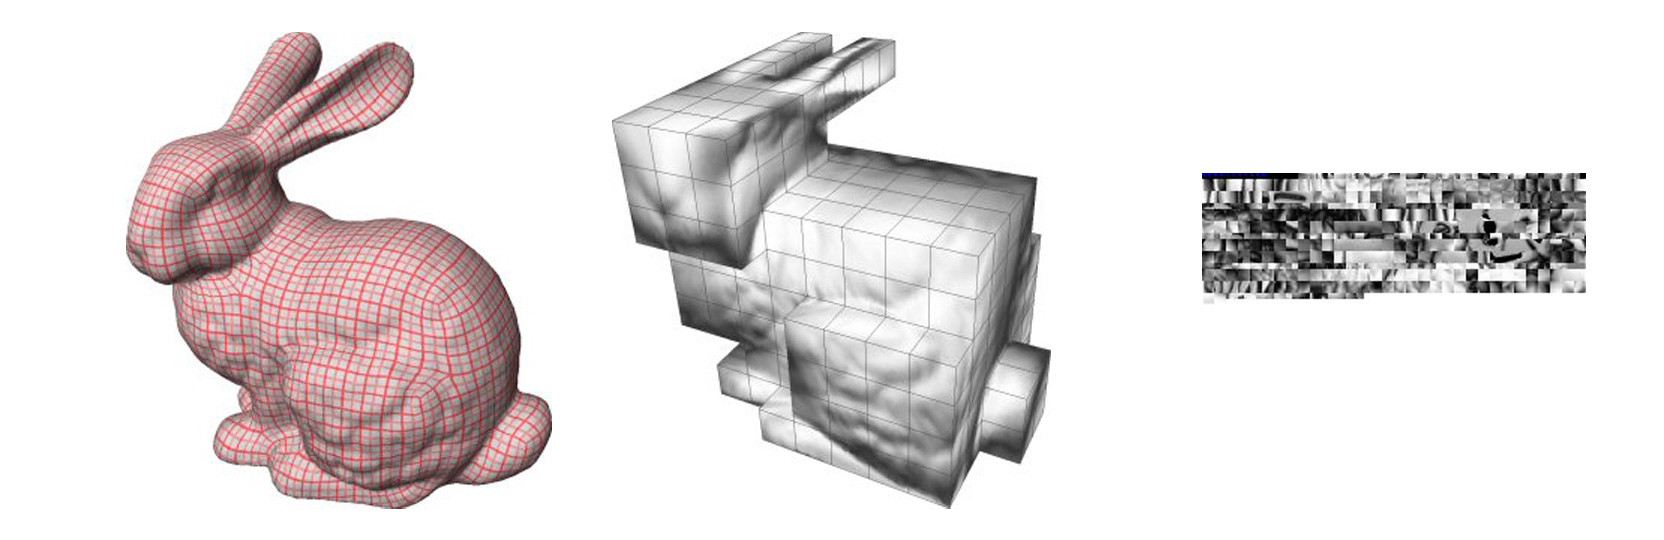
\includegraphics[width=\linewidth]{images/teaser}}

\begin{document}

\slidetitle
%\slidetableofcontents

%\slidesectionwithgraphic[bottom]{Cool Section Slide}{images/old_man}

\slideonetoone
{Initial Inspiration}
{
	\begin{figure}
		\centering
		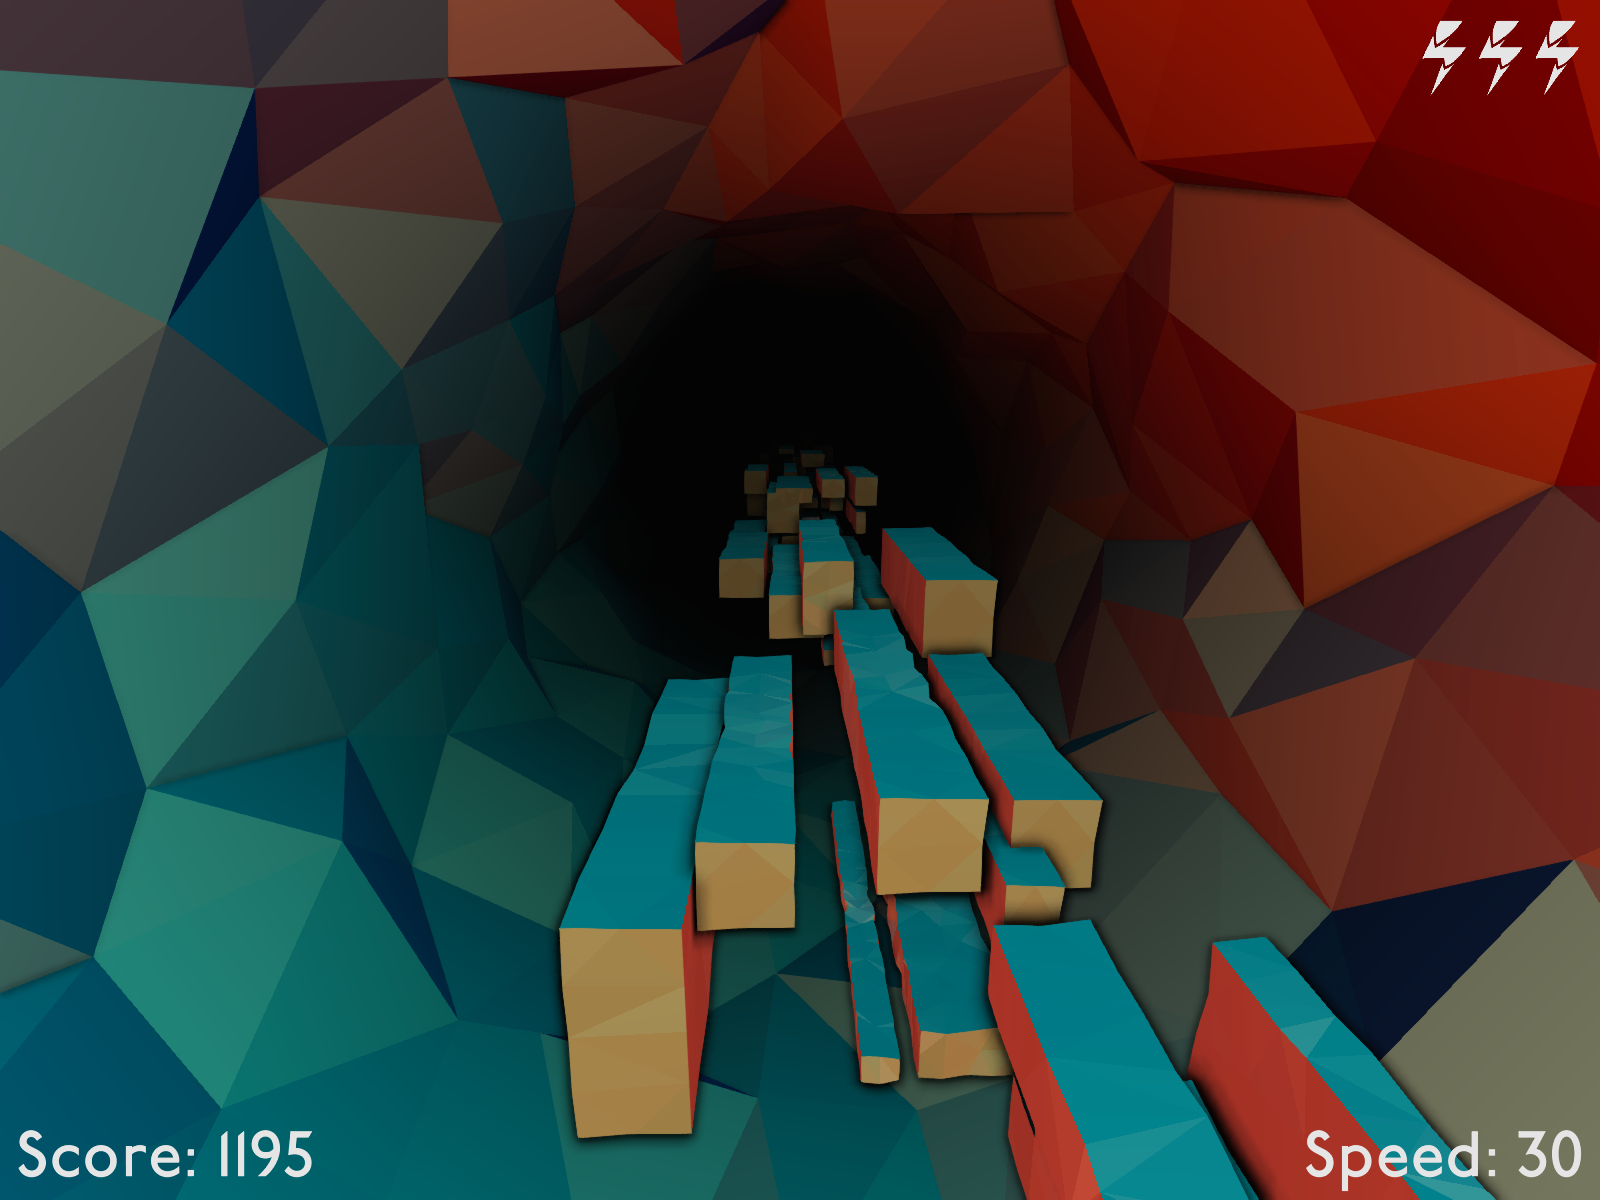
\includegraphics[width=\textwidth, height=0.7\textheight, keepaspectratio]{images/mammut_cave}
		\caption{Game Programming 2013/14: 
Mammut \linebreak A highspeed gravity racer}
	\end{figure}
}
{
	\begin{itemize}
		\item Spielerüberforderung ...
		 \begin{itemize}
		 	\item durch hohe Geschwindigkeit
		 	\item durch Perspektivenwechsel (Drehung um 90 Grad)
		 	\item durch Gravitationsänderung
		 \end{itemize}
		 \item Cartoonähnliche Grafik 
		 \item Wenige Farbtöne
	\end{itemize}
}

\slideonetoone
{Initial Inspiration}
{
	\begin{figure}
		\centering
		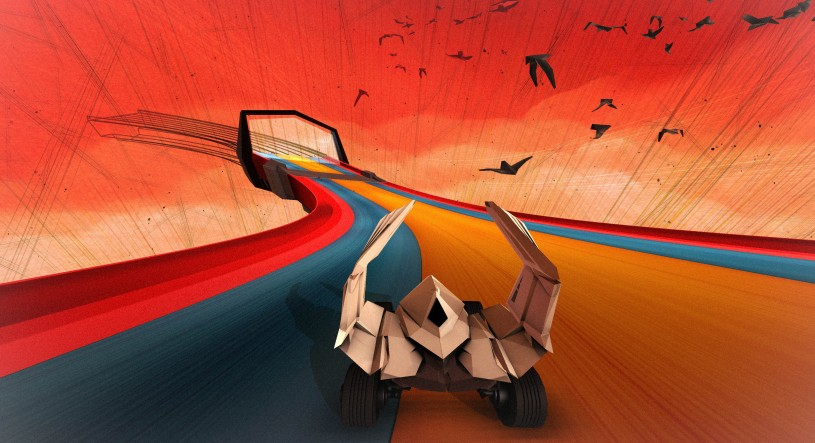
\includegraphics[width=\textwidth, height=0.7\textheight, keepaspectratio]{images/krautscape_ks1}
		\caption{Krautscape \linebreak Multiplayer racing with procedural tracks}
	\end{figure}
}
{
	\begin{itemize}
		\item Prozedurale Streckengenerierung
		\item Beeinflussung der Streckengenerierung durch den Spieler
		\item Hohe Geschwindigkeit
		\item Cartoonähnliche Grafik
	\end{itemize}
}

\slideonetoone
{Idea Development}
{
	\begin{itemize}
		\item Abstraktes Konzept:
		\begin{itemize}
			\item Start und Ziel im Raum
			\item Schwebender Torus als Spielfigur auf der Strecke
			\item Prozedurale Streckengenerierung durch den Spieler
			\item Items und Powerups für Effekt
		\end{itemize}
		\item Wir sind die Strecke?
		\item Wir sind das Licht?
		\item Wir sind Licht!
		\item Erzeugen eines Bildes
		\item Lichtsteuerung durch Kristalle
		\item Einfärben von Kristallen
	\end{itemize}
}
{
	\begin{figure}
		\centering
			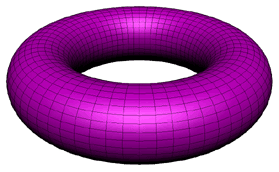
\includegraphics[width=\textwidth, height=0.2\textheight, keepaspectratio]{images/primitive_torus}
	\end{figure}
	\begin{figure}
		\centering
		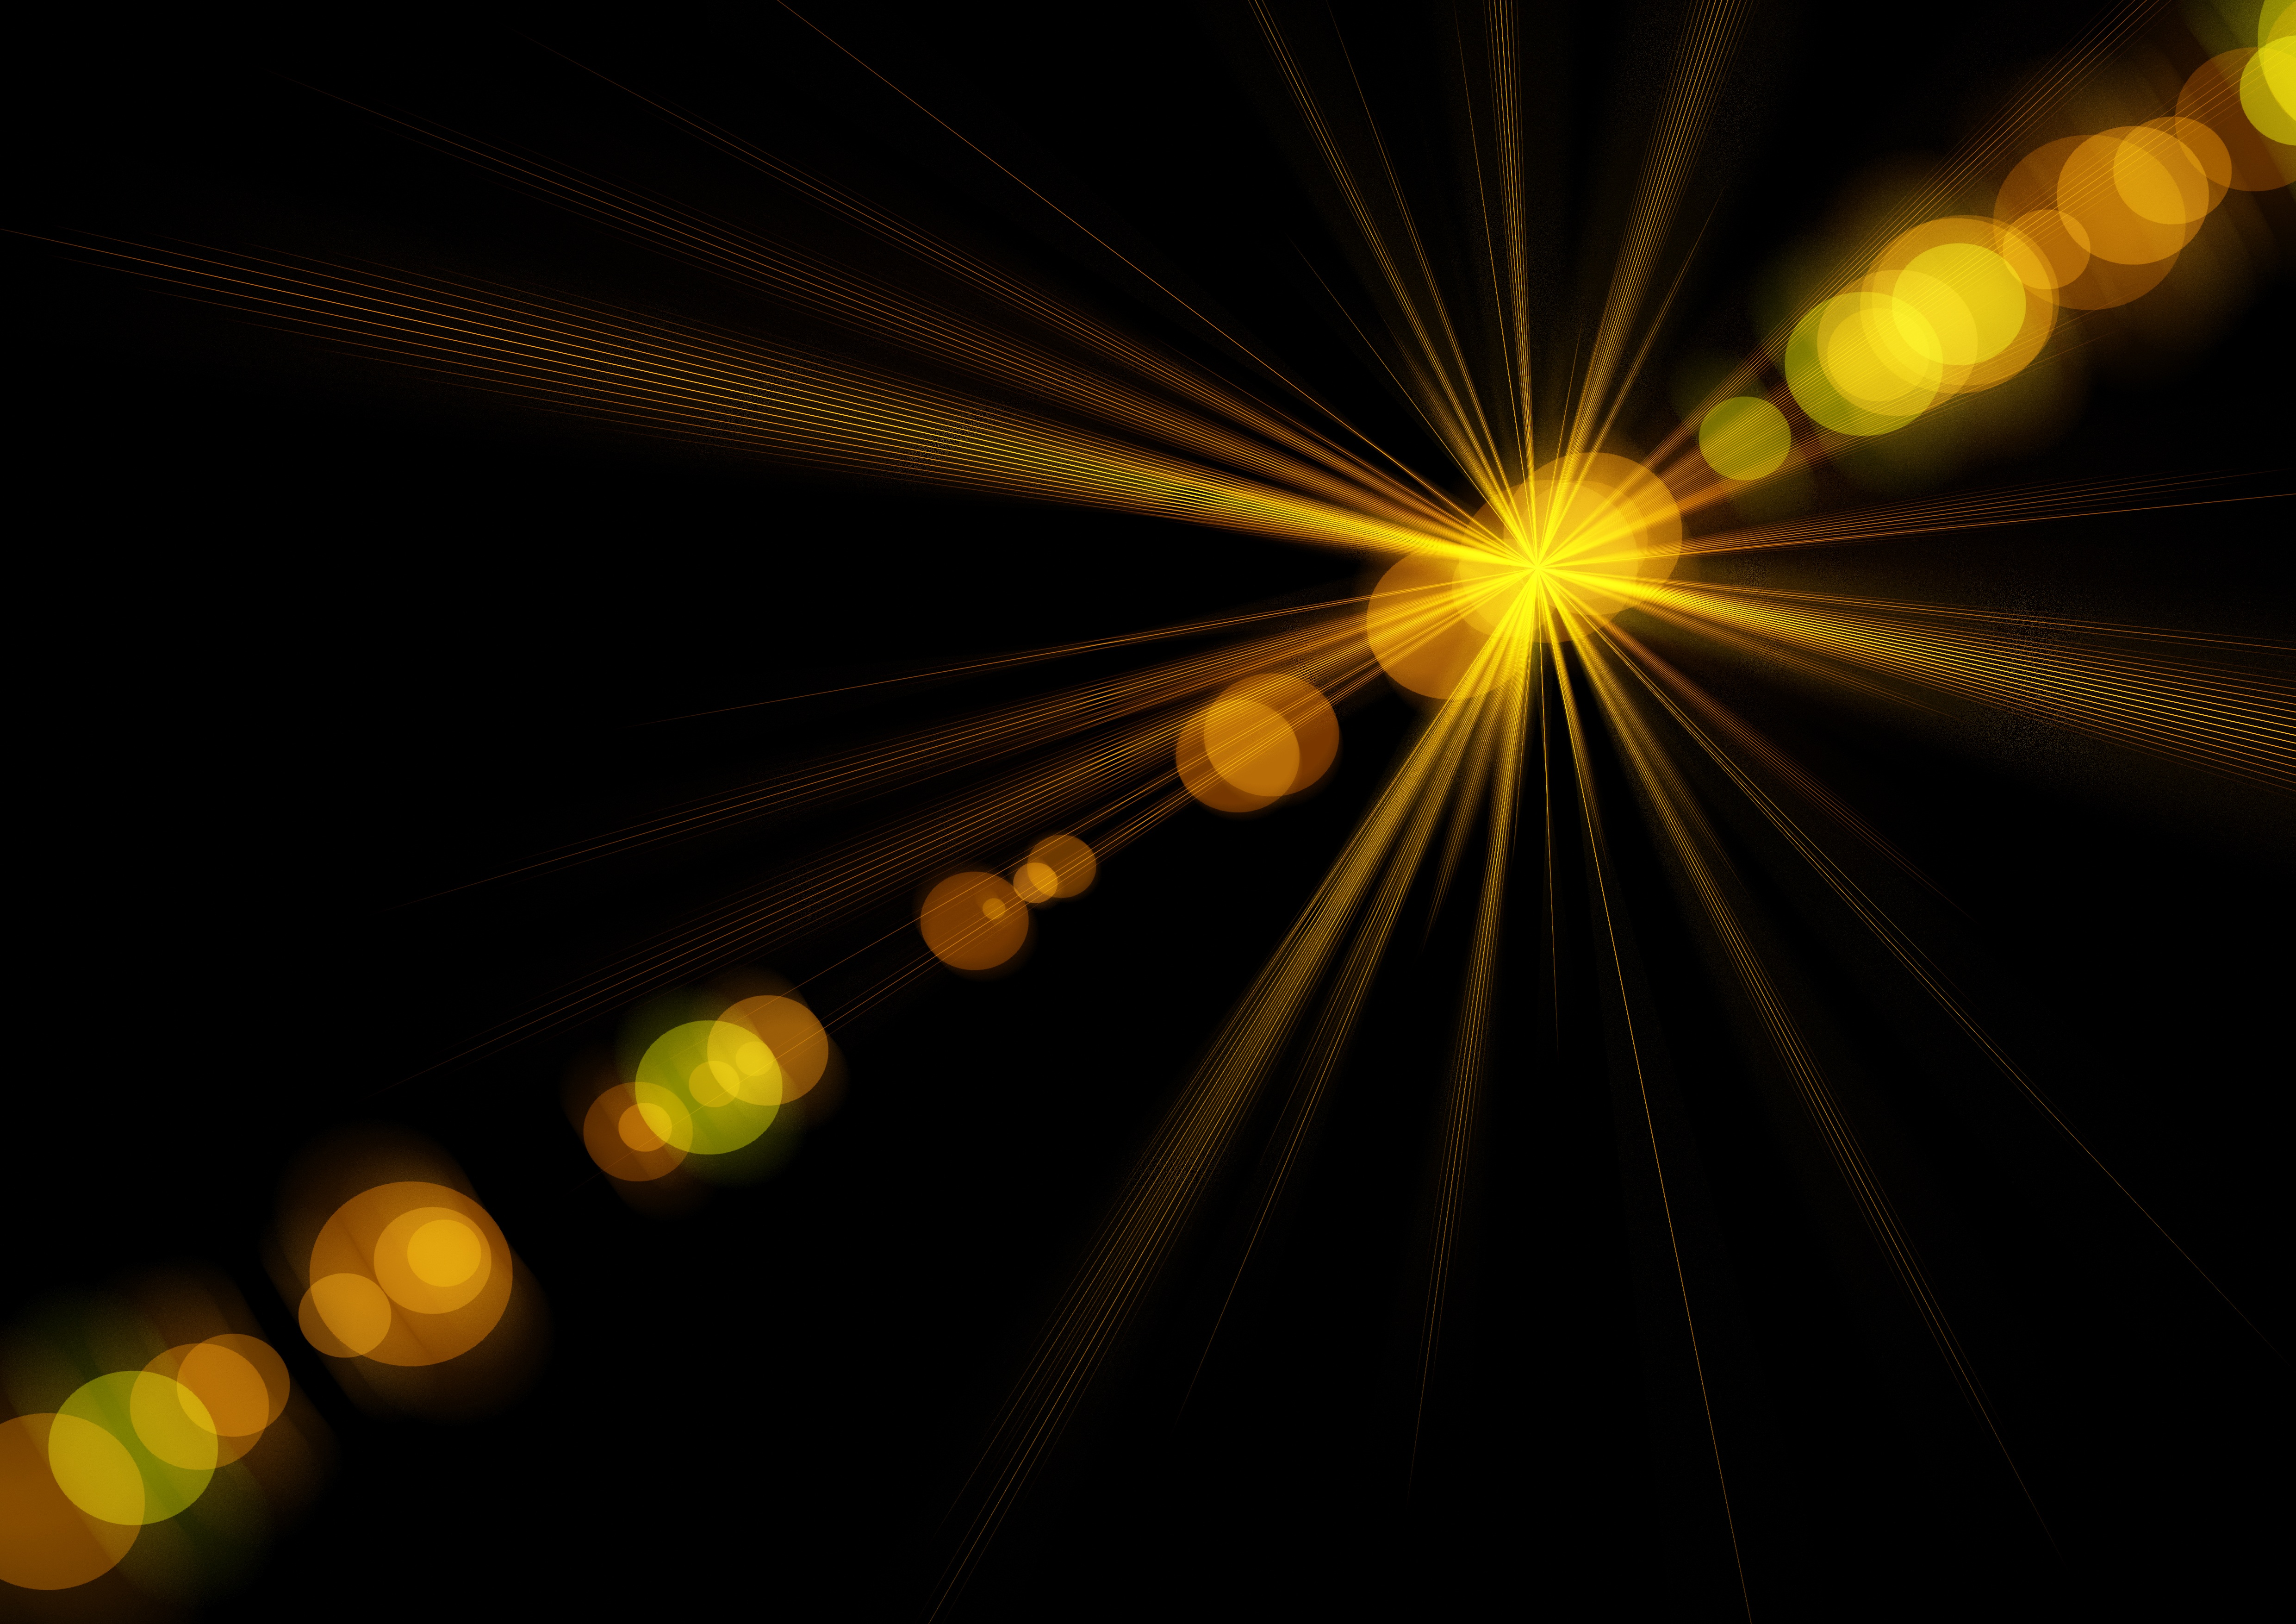
\includegraphics[width=\textwidth, height=0.2\textheight, keepaspectratio]{images/bokeh-419869}
	\end{figure}
	\begin{figure}
		\centering
		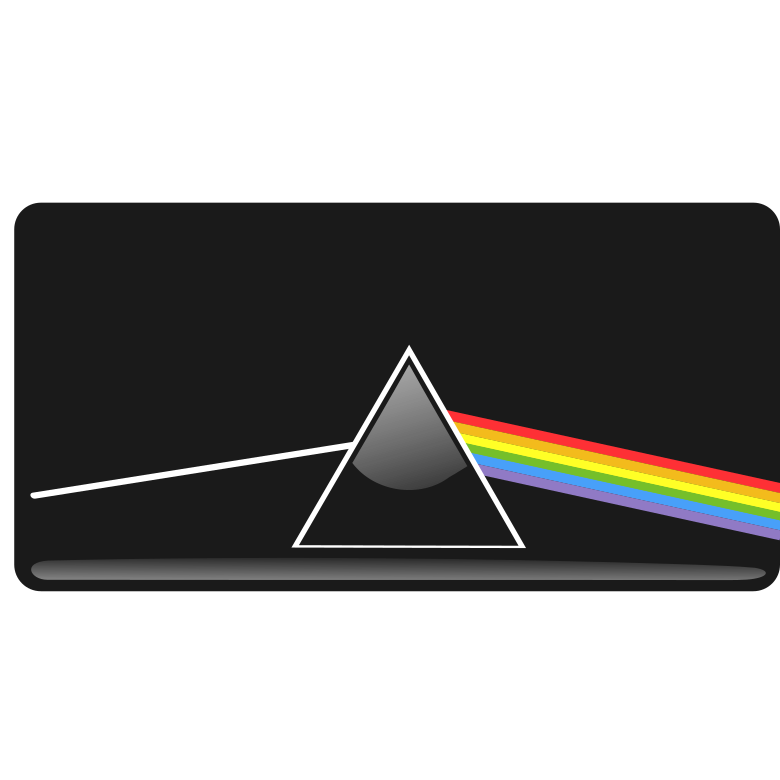
\includegraphics[width=\textwidth, height=0.2\textheight, keepaspectratio]{images/refraction-150853}
	\end{figure}
}

\begin{frame}{Must Have}
	\onetoone
	{
	\begin{itemize}
		\item Einfärben der Kristalle
		\item Kristalllandschaft
		\item Steuerung des nächsten Kristalls
		\item Energielevel des Lichtstrahls
	\end{itemize}
	}
	{
		\begin{figure}
			\centering
			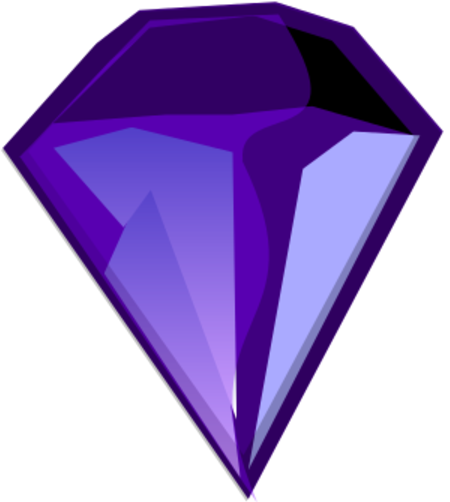
\includegraphics[width=\textwidth, height=0.3\textheight, keepaspectratio]{images/diamond-308079}
		\end{figure}
	}
	\begin{figure}
		\centering
		
\includegraphics[width=\textwidth, height=0.7\textheight, keepaspectratio]{images/chalk-154720}
	\end{figure}
\end{frame} 

\begin{frame}{Should Have}
	\onetoone
	{
		\begin{itemize}
			\item Perspektivenwechsel um mindestens 90$^\circ$
			\item Berechnung und Hervorhebung des übernächsten Kristalls
			\item Hindernisse
			\item Verschiedene Kristalle/Kristalleigenschaften
		\end{itemize}
	}
	{
		\begin{figure}
			\centering
			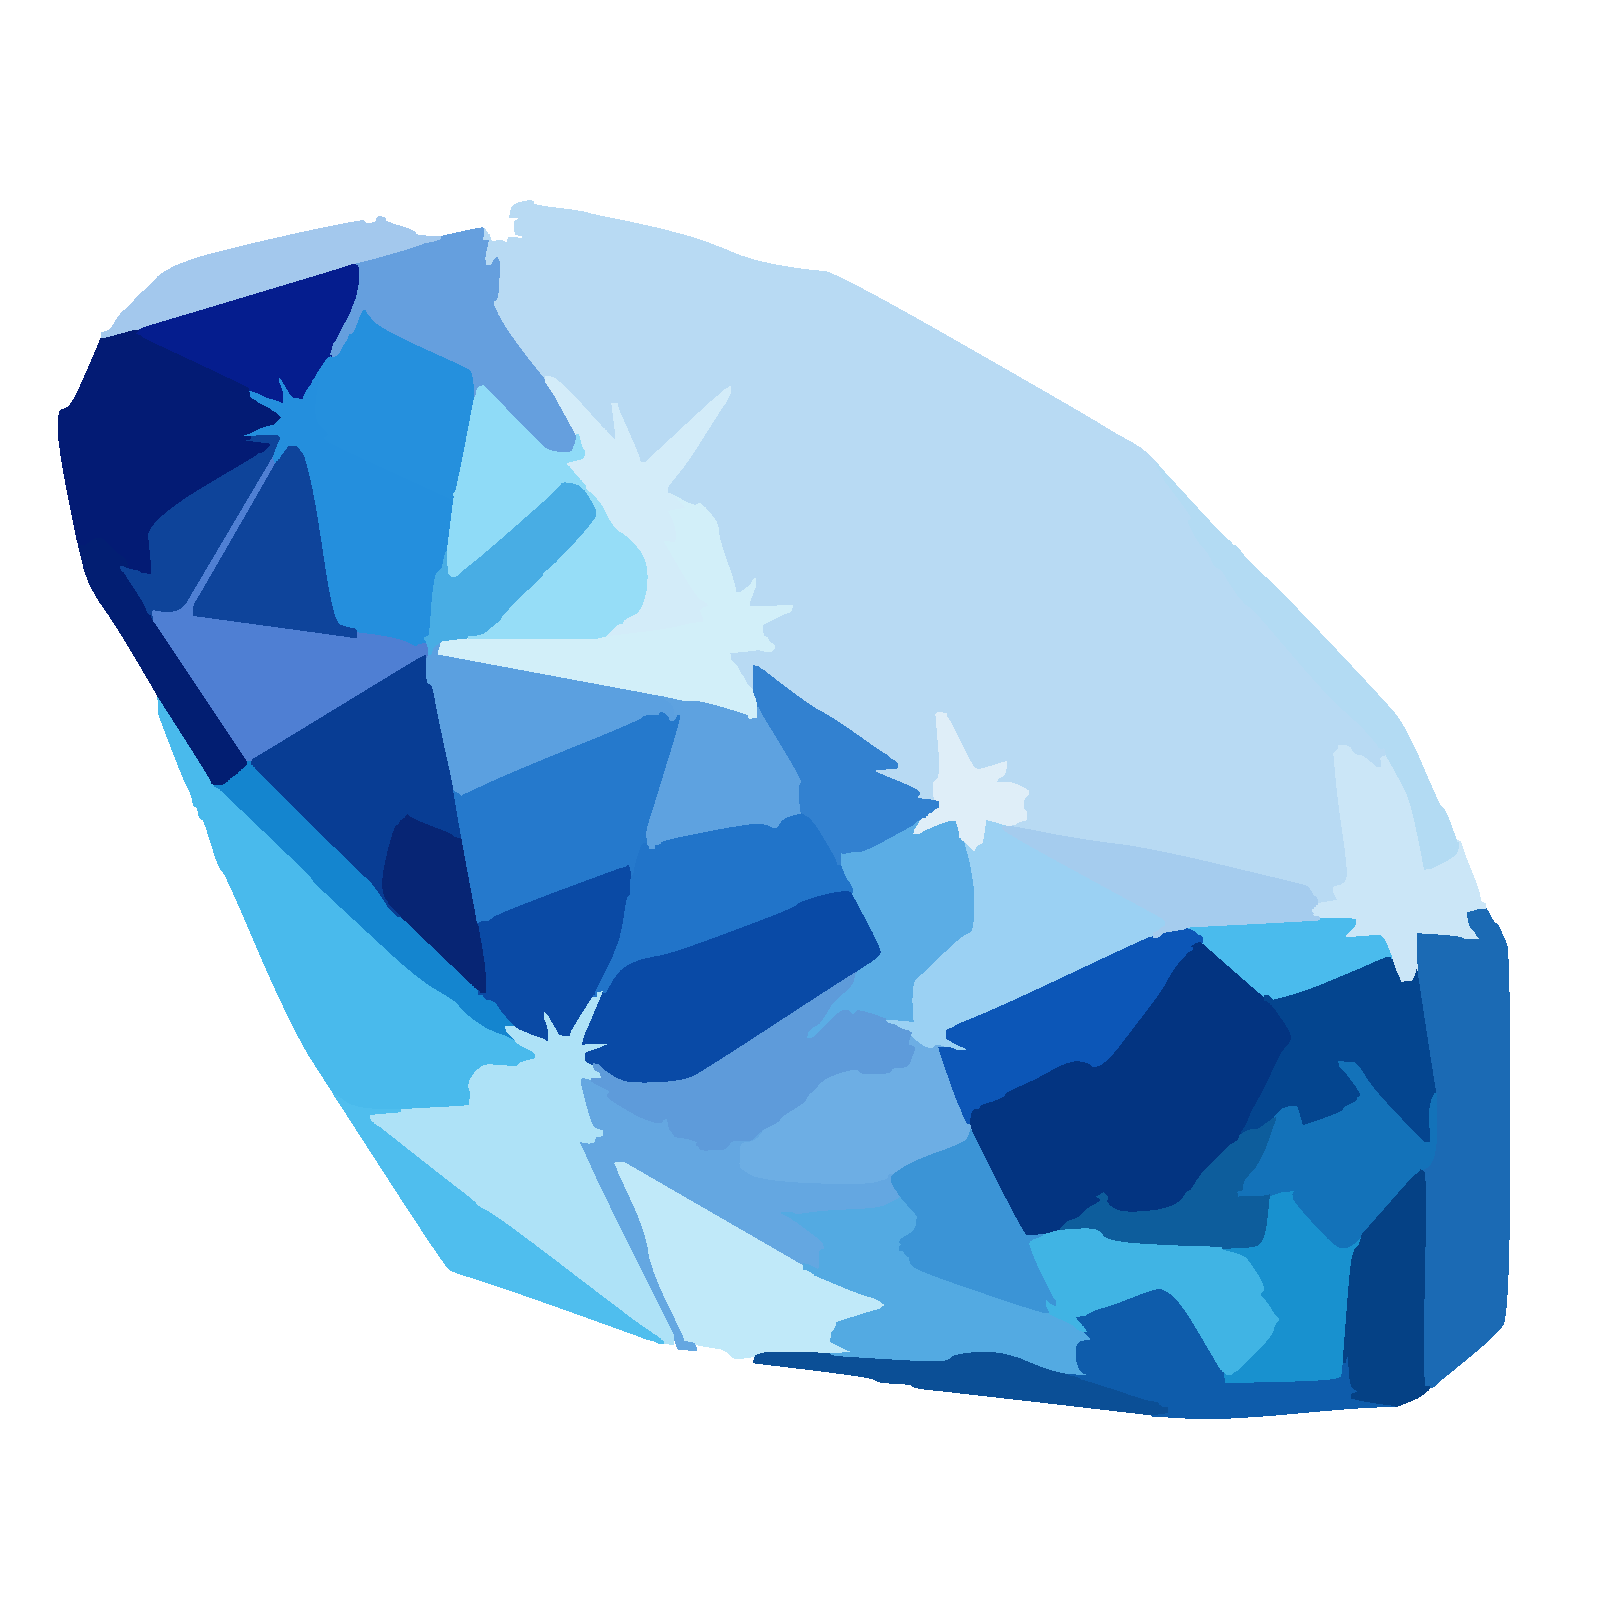
\includegraphics[width=\textwidth, height=0.4\textheight, keepaspectratio]{images/diamond-304884}
		\end{figure}
	}
	\begin{figure}
		\centering
		\begin{subfigure}{0.45\textwidth}
			\centering
			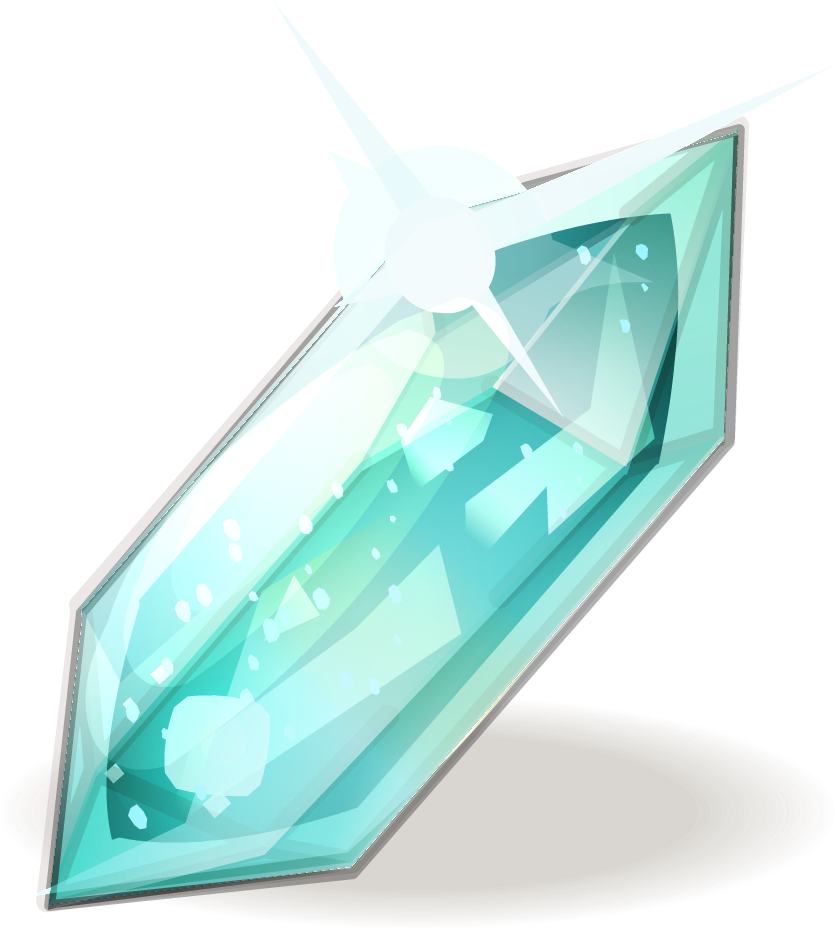
\includegraphics[width=\textwidth, height=0.3\textheight, keepaspectratio]{images/Resonanz-Kristall}
		\end{subfigure}
		\begin{subfigure}{0.45\textwidth}
			\centering
			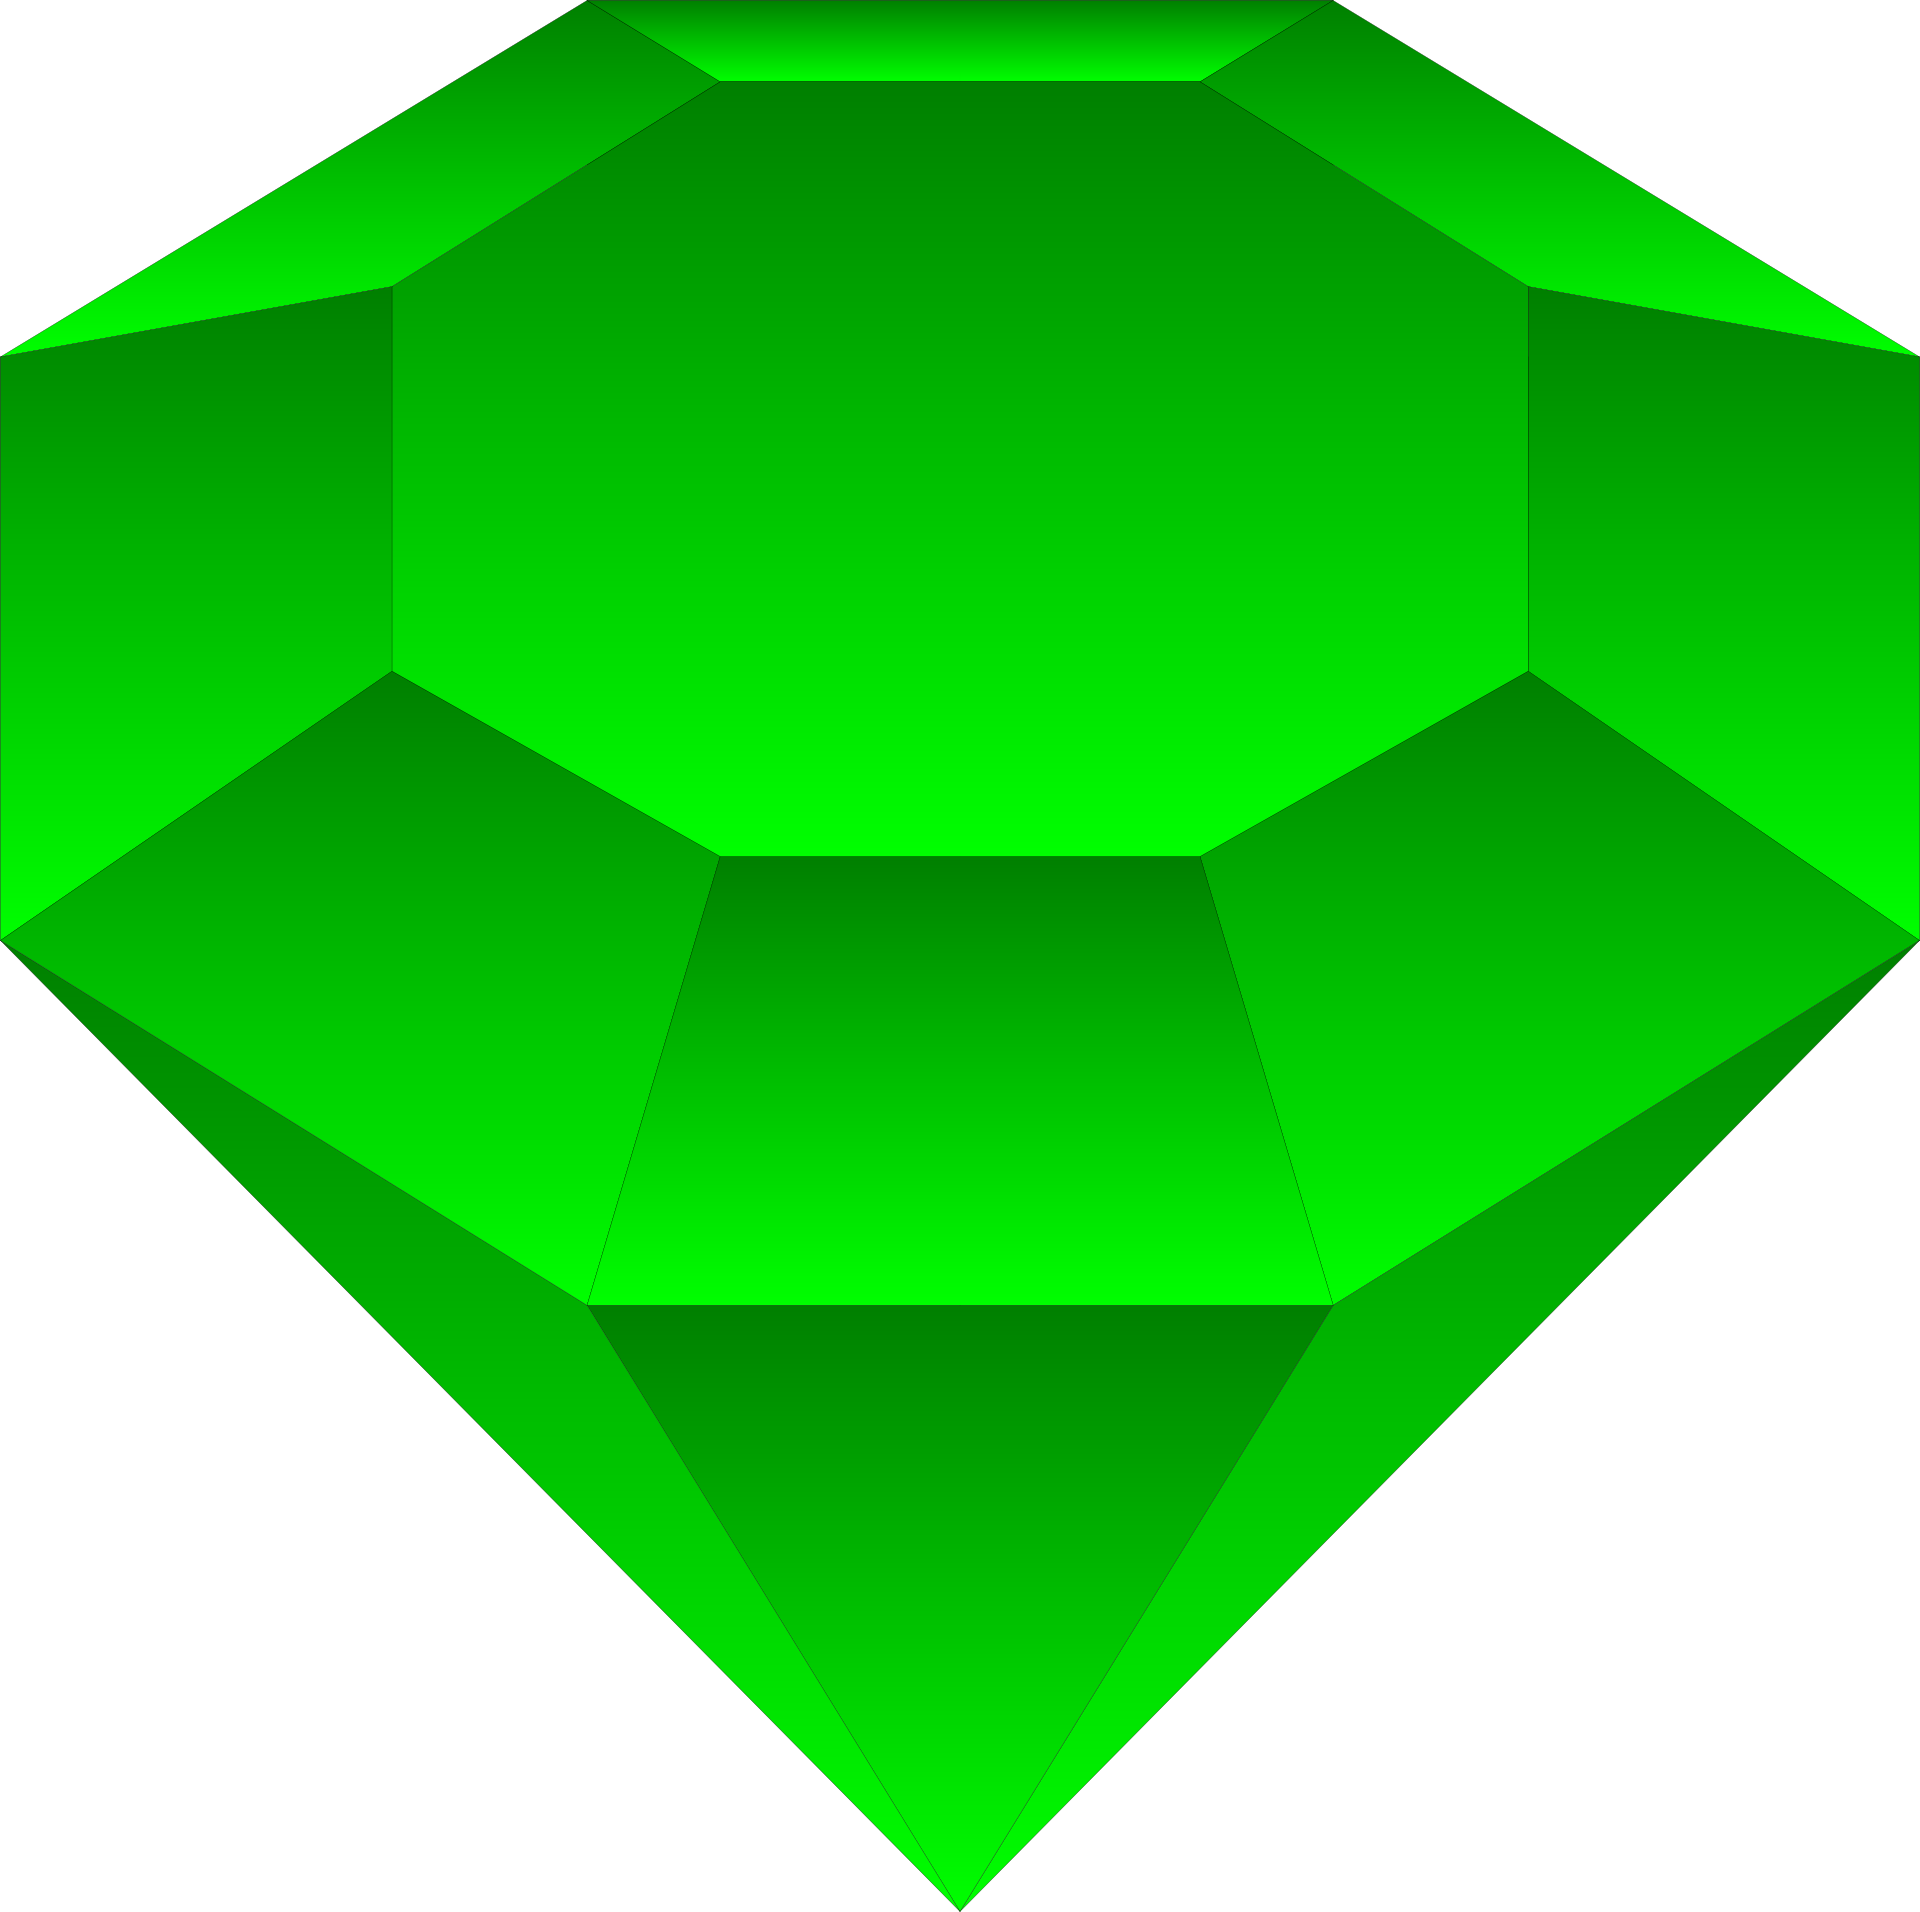
\includegraphics[width=\textwidth, height=0.3\textheight, keepaspectratio]{images/diamond-309694}
		\end{subfigure}
	\end{figure}
\end{frame}

\slideonetoone
{Nice to Have}
{
	\begin{itemize}
		\item Wissenschaftlichbasiertes Lichtmodell 
		\item Wissenschaftlichbasiertes Farbmodell
		\item Erstellen der Kristalllandschaft durch das Herunterfallen einer Schmuckkassette
		\item Intro, bei dem man den Lichtstrahl von der Sonne zur Erde verfolgt
		\item Spielende: Umwandlung der Kristalle in Würfel
	\end{itemize}
}
{
	\begin{figure}
		\centering
		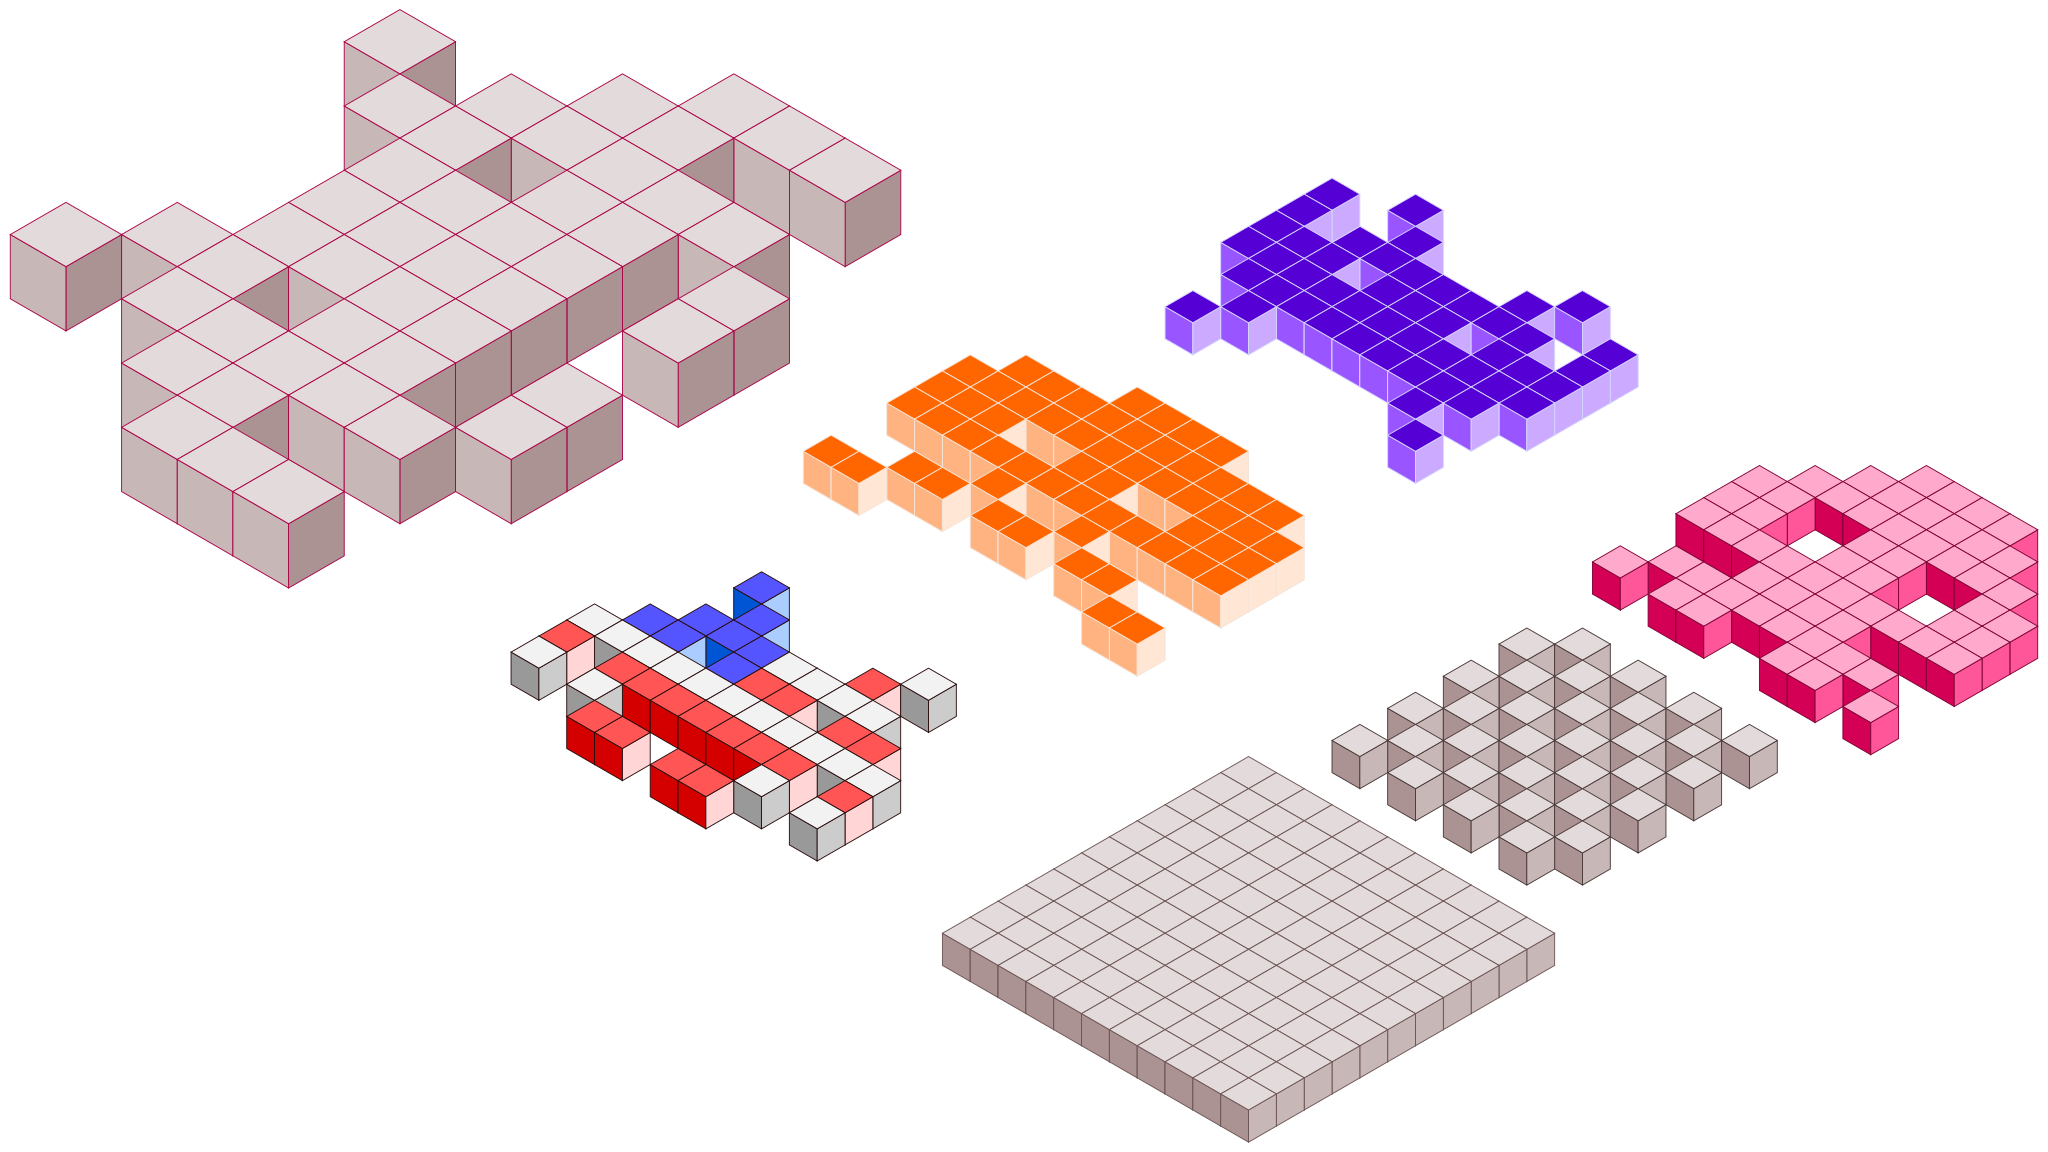
\includegraphics[width=\textwidth, height=0.7\textheight, keepaspectratio]{images/space-invaders-151432}
	\end{figure}
}

%\begin{frame}[allowframebreaks]{Bibliographie}
  \bibliographystyle{apalike}
  \bibliography{../../references}
  \vfill
\end{frame}

\end{document}
